\documentclass[11pt, titlepage]{article} 

\usepackage{geometry}
\geometry{left=0.8in, right=0.8in, top=0.8in, bottom=0.8in}

\usepackage{color}
\usepackage{graphicx} % slike
\usepackage{caption}
\usepackage{subcaption}
\usepackage{siunitx} % enote
\usepackage{amsmath} % enačbe
\usepackage{amssymb} % simboli
\usepackage[thinc]{esdiff} % za odvode
\usepackage[colorlinks=true]{hyperref} % za linke
\usepackage{float} % za fiksiranje figur
\usepackage{mathtools}
\usepackage{esint} % za fancy integrale
\usepackage[numbib,nottoc]{tocbibind}
\usepackage[slovene]{babel}


\usepackage{tikz}

\newcommand{\dif}[1]{\,{\rm d}#1}

\begin{document}

\begin{titlepage}
    \begin{center}
        \includegraphics[width=0.5\textwidth]{figures/FRI_logo.png}\\
        \vspace{0.5cm}
        \vspace{3cm}
        {\LARGE \bf QR razcep simetrične tridiagonalne matrike} \\
        \vspace{0.3cm}
        \vspace{2.0cm}
        {\large Numerična matematika}\\
        \vspace{0.2cm}
        {|}\\
        \vspace{0.2cm}
        {\large 1. domača naloga}\\
        \vspace{2.0cm}
    \end{center}
    \vfill
    \begin{flushleft}
        {\normalsize {\sf Avtor:} Vito Levstik\\}
    \end{flushleft}
    \vspace{2cm}
    \begin{center}
        {\normalsize \sc Akademsko leto 2024/2025}
    \end{center}
\end{titlepage}

\newpage

\section{Uvod}

Cilj te naloge je implementirati učinkovit QR razcep (simetrične) tridiagonalne matrike z Givensovimi rotacijami 
in ga uporabiti pri QR iteraciji za izračun lastnih vrednosti in lastnih vektorjev simetrične tridiagonalne matrike.

Da to dosežemo, implementiramo naslednje tipe: \texttt{Tridiag}, ki predstavlja tridiagonalno matriko,
\texttt{SimTridiag}, ki predstavlja simetrično tridiagonalno matriko, \texttt{Givens}, ki predstavlja matriko Givensovih rotacij in
\texttt{ZgornjeTridiag}, ki predstavlja matriko z neničelnimi elementi na diagonali in dveh zgornjih diagonalah.

Glavna naloga je tako implementacija funkcije \texttt{qr($T$)}, ki tridiagonalno matriko $T$ razcepi v produkt matrik $Q$ in $R$, kjer je $Q$ tipa \texttt{Givens} in $R$ tipa \texttt{ZgornjeTridiag} in
implementacija funkcije \texttt{eigen($T$)}, ki izračuna lastne vrednosti in lastne vektorje simetrične tridiagonalne matrike $T$ z uporabo QR iteracije.

\section{Implementacija}
Podatkovni tip \texttt{Tridiag} sprejme tri sezname in sicer seznam spodnje diagonale, seznam glavne diagonale in seznam zgornje diagonale.
Koda za tale tip je povzeta iz vaj. Podatkovni tip \texttt{SimTridiag} je podobno definiran, le da sprejme dva seznama, seznam glavne diagonale in seznam pod-diagonale, 
saj sta zgornja in spodnja diagonala enaka. Podatkovni tip \texttt{ZgornjeTridiag} je podoben, le da sprejme seznam glavne diagonale in dva seznama zgornjih diagonal.

Do elementov vseh treh matrik lahko dostopamo z indeksi, kot pri običajni matriki, kar smo storili z implementacijo funkcij \texttt{getindex()}. Elemente matrik lahko tudi spreminjamo s funkcijo \texttt{setindex()},
vendar to lahko naredimo le za elemente, ki so v matriki definirani. V nasprotnem primeru, bo program vrnil napako.

Pomemben podatkovni tip, ki si zasluži bolj podroben opis je \texttt{Givens}. Ta podatkovni sprejme seznam 4-dimenzionalnih vektorjev. Prvi dve komponenti sta kosinus $c$ in sinus $s$ kota rotacije, medtem ko sta tretja in četrta komponenta
indeksa $i$ in $j$ stolpcev/vrstic, ki jih rotiramo. V našem problemu se $i$ in $j$ vedno pojavita kot zaporedni števili, kar nam olajša določena množenja, zato bi lahko poenostavili ta tip, vendar da ohranimo splošnost, smo ga implementirali tako. 
Za boljšo predstavo si poglejmo matrično reprezentacijo Givensove rotacije
\[
G(c,s,i,j) =
\begin{bmatrix}
1      & \cdots & 0      & \cdots & 0      & \cdots & 0      \\
\vdots & \ddots & \vdots &        & \vdots &        & \vdots \\
0      & \cdots & c      & \cdots & -s     & \cdots & 0      \\
\vdots &        & \vdots & \ddots & \vdots &        & \vdots \\
0      & \cdots & s      & \cdots & c      & \cdots & 0      \\
\vdots &        & \vdots &        & \vdots & \ddots & \vdots \\
0      & \cdots & 0      & \cdots & 0      & \cdots & 1      
\end{bmatrix}
\]
kjer se $c = \cos(\theta)$ in $s = \sin(\theta)$, kjer je $\theta$ kot rotacije, pojavita na presečišču $i$ in $j$-te vrstice in stolpca.

V splošnem moramo pri QR razcepu eliminirati elemente pod glavno diagonalo. Ključno opažanje pri razcepu tridiagonalne matrike je, da so elementi potrebni eliminacije samo elementi spodnje diagonale.
To nam da motivacijo, da implementiramo funkcijo v časovni zahtevnosti $O(n)$, saj imamo samo $n-1$ elementov za eliminirati. Le-te lahko eliminiramo z uporabo Givensovih rotacij.
Konkretno, če želimo eliminirati $a_{i+1,i}$ v matriki $A$, se ga lahko znebimo tako, da pomnožimo $A$ iz leve z Givensovo rotacijo $G(c,s,i,i+1)$. Pri tem je potrebno izbrati ustrezen $c$ is $s$.
Izkaže se, da je
$$
c = \frac{a_{i,i}}{\sqrt{a_{i,i}^2 + a_{i+1,i}^2}}, \qquad s = \frac{a_{i+1,i}}{\sqrt{a_{i,i}^2 + a_{i+1,i}^2}}.
$$ 

Ko pomnožimo $A$ z Givensovo rotacijo $G(c,s,i,i+1)$ smo s tem izničili $a_{i+1,i}$, spremenili elemente $a_{i,i}$, $a_{i+1,i+1}$, $a_{i,i+1}$ in $a_{i+1,i+2}$, ter ustvarili nov neničeln element $a_{i,i+2}$ (pod predpostavko da so vsi elementi spodnje diagonale pred $a_{i+1,i}$ že eliminirani). Ta novo nastali element je element zgornje druge nad-diagonale.
To pomeni, da celoten algoritem QR razcepa tridiagonalne matrike operira le na spodnji diagonali, glavni diagonali in dveh zgornjih diagonalah.
Algoritem je tako preposto enojna zanka po vseh elementih spodnje diagonale, kjer za vsak element izračunamo ustrezno Givensovo rotacijo, posodobimo elemente po množenju in dodamo Givensovo rotacijo v seznam rotacij.
Končen rezultat je tako matrika $R$ tipa \texttt{ZgornjeTridiag} in matrika $Q$ tipa \texttt{Givens}, ki je produkt vseh Givensovih rotacij, ki smo jih uporabili pri eliminaciji.

Za QR iteracijo potrebujemo funkcijo množenja med matrikami tipa \texttt{Givens} in \texttt{ZgornjeTridiag}. Ko bodisi z leve ali desne pomnožimo matriko tipa \texttt{ZgornjeTridiag}
z matriko tipa \texttt{Givens}, v splošnem ni nujno, da je dobljena matrika v obliki katerega od definiranih tipov. S QR razcepom tridiagonalne matrike dobimo matriko $R$ tipa \texttt{ZgornjeTridiag} in matriko $Q$ tipa \texttt{Givens}, torej je v našem
primeru produkt $QR$ matrika tipa \texttt{Tridiag}. Izkaže se, da je ob QR razcepu simetrične tridiagonalne matrike produkt $RQ$ prav tako matrika tipa \texttt{SimTridiag}. Množenje med matrikami tipa \texttt{Givens} in \texttt{ZgornjeTridiag} je zato implementirano tako,
da se privzame, da je rezultat množenja matrika tipa \texttt{Tridiag}. Da se ohrani splošnost implementacije tudi v primeru, ko rezultat ni matrika tipa \texttt{Tridiag}, se med množenjem preveri, ali so kateri elementi izven stranskih diagonal neničelni.
V tem primeru se zgornje tridiagonalna matrika pretvori v polno matriko in se nato izvede množenje.

Lastne vrednosti in lastne vektornje simetrične tridiagonalne matrike dobimo z uporabo QR iteracije. Algoritem QR iteracije je sledeč. Simetrično tridiagonalno matriko $T$ razcepimo v produkt $T = QR$, z že implementirano funkcijo \texttt{qr($T$)}.
Pri tem si shranimo matriko $Q$ in nato izračunamo $T = RQ$, ki je ponovno simetrično tridiagonalna. Ta postopek ponavljamo poljubno število korakov. Elementi na diagonali matrike $T$ konvergirajo v lastne vrednosti, medtem ko so pripadajoči lastni vektorji stolpci matrike dobljene kot produkt vseh matrik $Q$.

\section{Rezultati}
Primerjamo QR razcep simetrične tridiagonalne matrike različnih velikosti z QR razcepom iz knjižice \texttt{LinearAlgebra}, ki operira na polni matriki. Rezultati so prizakani na sliki \ref{fig:qr_comparison}.
\begin{figure}[ht]
    \centering
    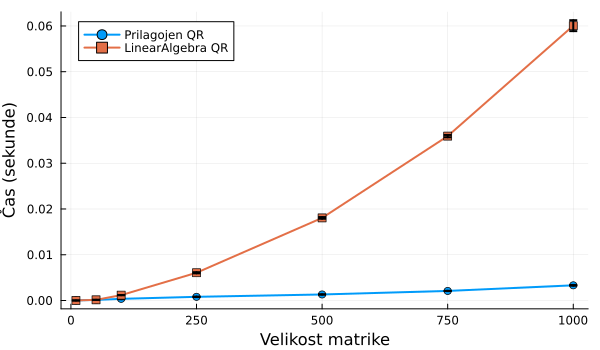
\includegraphics[width=0.7\textwidth]{figures/qr_performance_comparison.png}
    \caption{Primerjava našega QR razcepa simetrične tridiagonalne matrike z QR razcepom iz knjižice LinearAlgebra.}
    \label{fig:qr_comparison}
\end{figure}

Vidimo, da je naš algoritem QR razcepa bistveno hitrejši pri večjih matrikah. Razlog je v tem, da je naš algoritem optimiziran za tridiagonalne matrike in deluje v $O(n)$, medtem ko QR razcep iz knjižice \texttt{LinearAlgebra} deluje za poljubne matrike, kar pomeni, da deluje v $O(n^3)$.
Po sliki sodeč naš algoritem resnično deluje v linearnem času, medtem ko QR razcep iz knjižice \texttt{LinearAlgebra} izgleda da deluje v bolj kompleksnem času (verjetno $O(n^3)$).

Za konec še poglejmo uporabo pri QR iteraciji simetrične tridiagonalne matrike. Za primer vzamemo matriko
$$
T = \begin{bmatrix}
    4 & 1 & 0 \\
    1 & 2 & 2 \\
    0 & 2 & 1
\end{bmatrix}.
$$
Analitična rešitev lastnih vrednosti te matrike so $\lambda_1 = 2 + \sqrt{7} \approx 4.6457513110645906$, $\lambda_2 = 3$ in $\lambda_3 = 2 - \sqrt{7} \approx -0.6457513110645906$.
Izvedemo QR iteracijo s $25$ koraki in dobimo lastne vrednosti $\lambda_1 \approx 4.645751289681215$, $\lambda_2 \approx 3.0000000213833773$ in $\lambda_3 \approx -0.645751311064591$.
Vidimo, da so lastne vrednosti zelo blizu analitičnim rešitvam, kljub majhnemu številu iteracij, kar pomeni, da QR iteracija zelo hitro konvergira. Na sliki \ref{fig:qr_iteration} je prikazana konvergenca lastnih vrednosti v odvisnosti od števila iteracij.
\begin{figure}[ht]
    \centering
    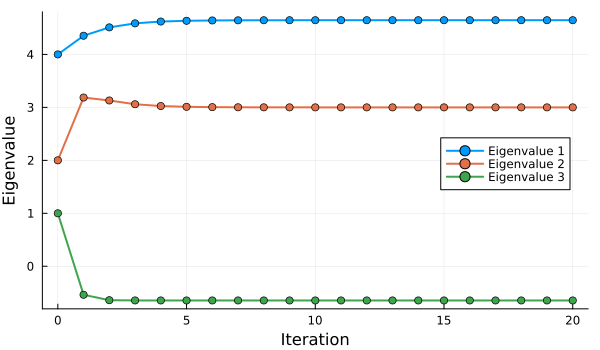
\includegraphics[width=0.7\textwidth]{figures/qr_iteration_convergence.png}
    \caption{Konvergenca lastnih vrednosti v odvisnosti od števila iteracij.}
    \label{fig:qr_iteration}
\end{figure}

\end{document}